\documentclass[journal=jcisd8,manuscript=article]{achemso}
\usepackage{graphicx}
\usepackage{xr-hyper}
\usepackage{hyperref}
\usepackage{xcolor}
\usepackage{verbatim}
\usepackage[subrefformat=parens]{subcaption}
\usepackage[finalizecache,cachedir=.]{minted}
\usepackage[version=3]{mhchem} % Formula subscripts using \ce{}

\renewcommand{\thetable}{S\arabic{table}}  
\renewcommand{\thefigure}{S\arabic{figure}}

\author{Paul G. Francoeur}
\author{David R. Koes}
\email{dkoes@pitt.edu}
\affiliation[Pitt]{Department of Computational and Systems Biology, University of Pittsburgh, Pittsburgh, PA 15260}

\title{Supporting Information:\\SolTranNet -- A machine learning tool for fast aqueous solubility prediction.}
\begin{document}
\begin{figure}[tb]
    \subfloat[Optimizer Hyperband Sweep]{
        \centering
        \begin{tabular}{|c|c|}
        \hline
            Parameter & Range \\
        \hline
            Training Epochs & [250, 2000]  \\
            Loss Function & MSE, MAE, Huber  \\
            Learning Rate & [0.0001, 0.1]  \\
            Momentum & [0.5, 0.9]  \\
            Optimizer & SGD, Adam  \\
            Weight Decay & [0, 0.5]  \\
            Dimension of Conformer Generation & 2D, 3D  \\
            Scaffold CCV fold & 0 \\
            Target & minimize test RMSE  \\
        \hline
        \end{tabular}
        \label{tab:initsweep}
    }
    
    \subfloat[Architecture Grid Search]{
        \centering
        \begin{tabular}{|c|c|}
        \hline
            Parameter & Range \\
        \hline
             Dimension of Conformer Generation & 2D, 3D  \\
             Latent Dimension of Encoder & 2, 4, \textbf{8}, 16, 32, 64, 128, 256, 512, 1024  \\
             Dropout & 0, \textbf{0.1}  \\
             Number of Attention Heads (\#Heads) & \textbf{2}, 4, 8, 16, 32  \\
             $\lambda_1$ Attention & 0.25, 0.33, \textbf{0.5}  \\
             $\lambda_2$ Distance & \textbf{0}, 0.33  \\
             Number of Encoder Stacks (\#Stacks) & 2, 4, 6, \textbf{8}, 16  \\
             Scaffold CCV folds & 0, 1, 2  \\
             Loss Function & Huber  \\
             Learning Rate & 0.04  \\
             Momentum & 0.06  \\
             Optimizer & SGD  \\
             Weight Decay & 0  \\
         \hline
        \end{tabular}
        \label{tab:archsweep}
    }
    \caption{Two stage hyperparameter sweep for SolTranNet. The Optimizer sweep was performed via using Weights and Bias's hyperband sweeping tool using Bayesian optimization (during which all values in ranges are considered), with the target to minimize the test set RMSE. The Architecture sweep was a grid search over the listed parameters after the optimizer hyperparameters were set from the first stage. The deployed version of SolTranNet uses the hyperparameters in bold.}
    \label{tab:wandsweep}
\end{figure}

\begin{table}
    %\centering
    \begin{tabular}{|c|c|c|c|c|c|c|}
        \hline
         Model & Parameters & CCV RMSE & Fold0 RMSE & Fold1 RMSE & Fold2 RMSE & Ind RMSE \\
         \hline
         MAT & 42,049,537 & 2.007 & 1.231 & 3.075 & 1.058 & 2.113  \\
         \hline
         0 & 21,061,633 & 1.449 & 1.161 & 1.959 & 1.054 & 1.914 \\
         1 & 502,529 & 1.467 & 1.231 & 1.972 & 1.028 & 1.946 \\
         2 & 336,385 & 1.377 & 1.260 & 1.682 & 1.126 & 1.870 \\
         3 & 336,385 & 1.454 & 1.239 & 1.857 & 1.165 & 1.949 \\
         4 & 22,657 & 1.297 & 1.187 & \textbf{1.582} & 1.066 & 1.903 \\
         5 & 11,905 & \textbf{1.271} & \textbf{1.130} & 1.605 & \textbf{0.998} & 1.923 \\
         6 & 11,905 & 1.350 & 1.272 & 1.680 & 1.012 & 1.903\\ \hline \hline
         7 & 3,393 & 1.459 & 1.172 & 1.916 & 1.159 & \textbf{1.779}\\ \hline \hline
         8 & 2,609 & 1.376 & 1.169 & 1.788 & 1.055  & 1.973 \\
         9 & 2,609 & 1.454 & 1.252 & 1.919 & 1.043  & 1.973 \\
         \hline \hline
         Elastic & 1,463 & 1.835 & 1.843 & 1.965 & 1.687  & 2.090\\
         Lasso & 1,077 & 1.876 & 1.914 & 1.984 & 1.719 & 2.136\\
         PLS & 2,048 & 2.413 & 3.085 & 2.082 & 1.902 & 2.081\\
         Ridge & 2,048 & 2.239 & 2.503 & 2.032 & 2.155 & 2.312 \\
         \hline
    \end{tabular}
    \caption{SolTranNet model hyperparameter search for predicting solubility RMSE on the scaffold-based clustered cross-validation splits of AqSolDB (CCV) and our independent test set (Ind). Additionally, all models outperform linear approaches trained on RDKit fingerprints using scikit-learn\cite{scikit-learn}. The isolated row (model 7) is the final SolTranNet architecture.}
    \label{tab:solsearchrmse}
\end{table}

\begin{table}
    %\centering
    \begin{tabular}{|c|c|c|c|c|c|c|}
        \hline
         Model & Parameters & CCV $R^2$ & Fold0 $R^2$ & Fold1 $R^2$ & Fold2 $R^2$ & Ind $R^2$ \\
         \hline
         MAT & 42,049,537 & 0.532 & 0.751 & 0.332 & 0.715 & 0.375  \\
         \hline
         0 & 21,061,633 & 0.670 & 0.778 & 0.520 & 0.727 & 0.4718 \\
         1 & 502,529 & 0.662 & 0.769 & 0.465 & 0.733 & 0.4576 \\
         2 & 336,385 & 0.693 & 0.764 & 0.563 & 0.706 & 0.4890 \\
         3 & 336,385 & 0.672 & 0.764 & 0.539 & 0.685 & 0.4461 \\
         4 & 22,657 & \textbf{0.724} & 0.780 & \textbf{0.626} & 0.716 & 0.4831 \\
         5 & 11,905 & \textbf{0.723} & \textbf{0.793} & 0.595 & 0.744 & 0.4628 \\
         6 & 11,905 & 0.713 & 0.786 & 0.582 & \textbf{0.756} & 0.4517 \\ \hline \hline
         7 & 3,393 & 0.6764 & 0.7914 & 0.5243 & 0.7424 & \textbf{0.5528}\\ \hline \hline
         8 & 2,609 & 0.695 & 0.779 & 0.545 & 0.737  & 0.4589\\
         9 & 2,609 & 0.677 & 0.767 & 0.552 & 0.720  & 0.4678\\
         \hline
         Elastic & 1,463 & 0.414 & 0.441 & 0.394 & 0.408  & 0.377\\
         Lasso & 1,077 & 0.395 & 0.409 & 0.378 & 0.392  & 0.351\\
         PLS & 2,048 & 0.228 & 0.212 & 0.333 & 0.0747  & 0.676\\
         Ridge & 2,048 & 0.319 & 0.289 & 0.354 & 0.291 & 0.261 \\
         \hline
    \end{tabular}
    \caption{SolTranNet hyperparameter search correlations. There is a general trend of models with fewer parameters performing better. Additionally, all models significantly outperform linear ML approaches. The isolated row (model 7) is the final SolTranNet.}
    \label{tab:solsearchr2}
\end{table}

\begin{table}
    %\centering
    \begin{tabular}{|c|c|}
        \hline
         Index & Description \\
         \hline
         0-11 & Atom Identity as one-hot (B,N,C,O,F,P,S,Cl,Br,I,Dummy,Other) \\
         12-17 & Number of heavy atom neighbors as one-hot of 0-5 \\
         18-22 & Number H atoms as one-hot of 0-4 \\
         23 & Formal Charge \\
         24 & In a Ring \\
         25 & Aromatic \\
         \hline
    \end{tabular}
    \caption{Featurization used to embed atoms in SolTranNet. This is the same schema as in the original MAT implementation. }
    \label{tab:atomembed}
\end{table}


\begin{figure}[tb]
    \centering
    \begin{subfigure}[t]{0.48\textwidth}
        \centering
        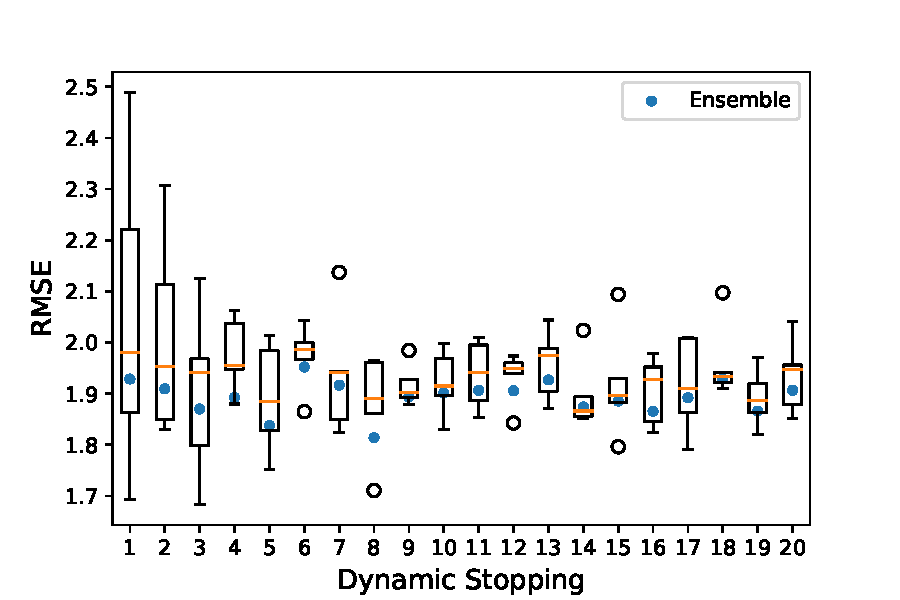
\includegraphics[width=\linewidth]{figures/final_model_ind_dyn_RMSE.pdf}
    \end{subfigure}%
    \hfill
    \begin{subfigure}[t]{0.48\textwidth}
        \centering
        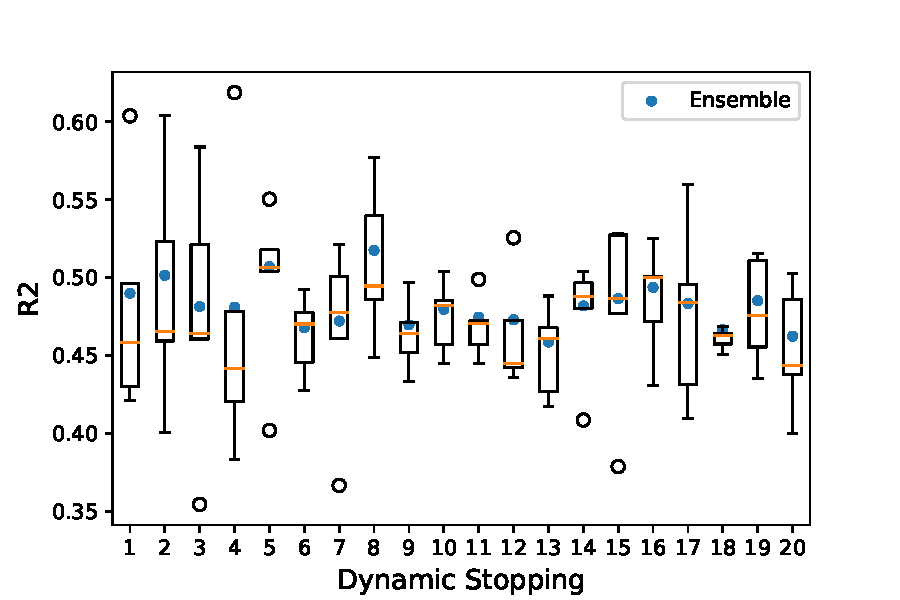
\includegraphics[width=\linewidth]{figures/final_model_ind_dyn_R2.pdf}
    \end{subfigure}
    \caption{Boxplots of the performance of SolTranNet models on our independent test set using various dynamic stopping criteria. The Dynamic Stopping is the number of epochs that the model can fail to improve its fit to the training set before training is stopped. The boxplot is of 5 different seeds, with the ensemble performance shown with the blue dot. Interestingly, the ensemble outperforms the mean performance of the 5 models, but fails to be better than the best performing seed in all cases.}
    \label{fig:dynsweep}
\end{figure}

\begin{table}
    \begin{tabular}{|c|c|c|c|c|}
        \hline
        Model & Train RMSE & Test RMSE & Train $R^2$ & Test $R^2$ \\
        \hline
        Average of 5 Seeds & 1.171 (0.0504) & 1.878 (0.0925)  & 0.784 (0.00643) & 0.509 (0.0445)\\
        Ensemble & \textbf{1.068} & 1.814 & \textbf{0.798} & 0.517\\
        Deployed & 1.144 & \textbf{1.711} & 0.777 & \textbf{0.577}\\
        \hline
    \end{tabular}
    \caption{Performance of 5 different seeds of SolTranNet. Each model was trained on all of AqSolDB and tested on our independent test set. The first row reports the mean and standard deviation (in parenthesis) for 5 models trained with different random seed. The second row is the ensemble performance of the models from the first row, with the final row being the results of the single best performing model. We note that the ensemble outperforms each model on average, but fails to beat the best performing seed. Deployed refers to the single best performing model.}
    \label{tab:deployed}
\end{table}

\begin{figure}[tb]
    \centering
    \begin{subfigure}[t]{0.48\textwidth}
        \centering
        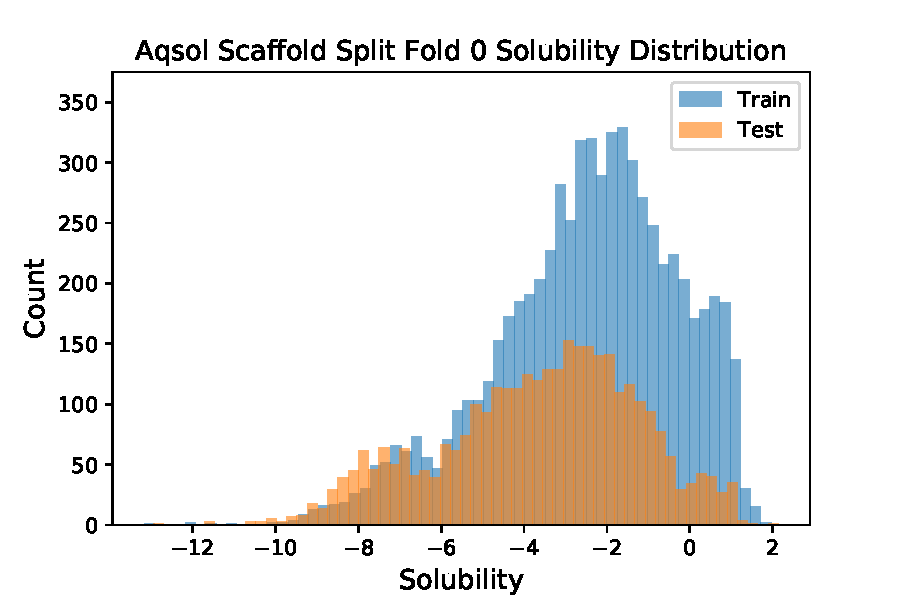
\includegraphics[width=\linewidth]{figures/aqsol_scaf0_soldist.pdf}
    \end{subfigure}%
    \hfill
    \begin{subfigure}[t]{0.48\textwidth}
        \centering
        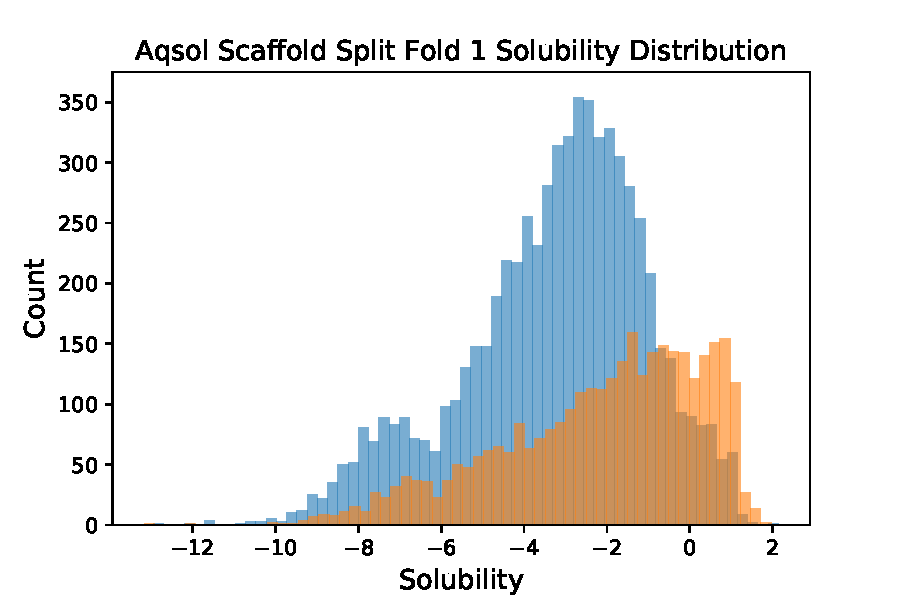
\includegraphics[width=\linewidth]{figures/aqsol_scaf1_soldist.pdf}
    \end{subfigure}
    
    \begin{subfigure}[t]{0.48\textwidth}
        \centering
        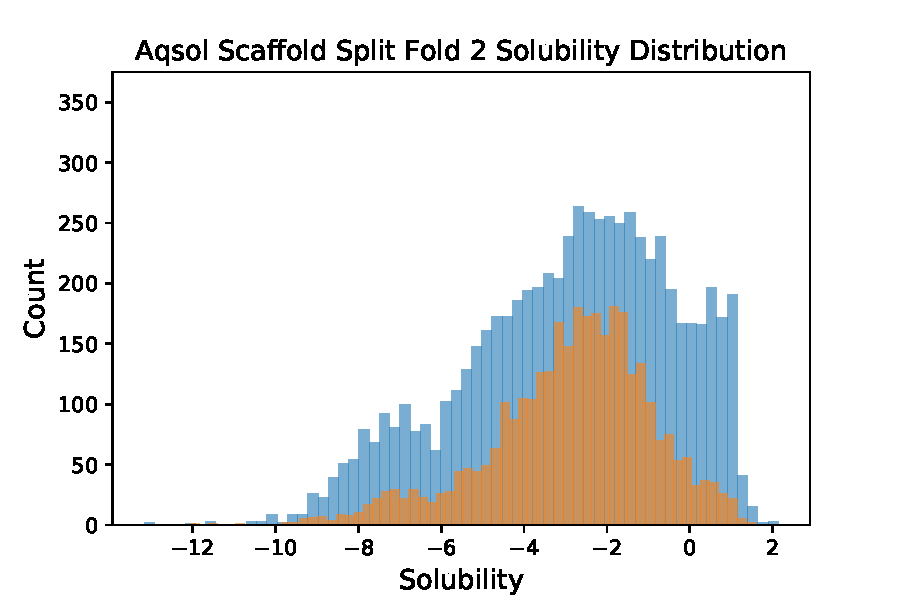
\includegraphics[width=\linewidth]{figures/aqsol_scaf2_soldist.pdf}
    \end{subfigure}
    
    
    \begin{subfigure}[t]{0.48\textwidth}
        \centering
        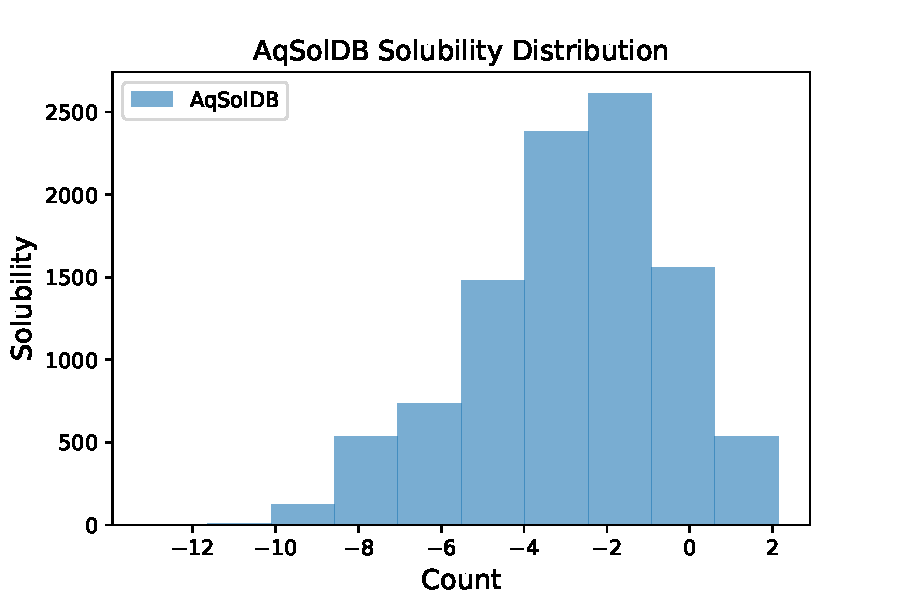
\includegraphics[width=\linewidth]{figures/AqSolDB_solhist.pdf}
    \end{subfigure}%
    \hfill
    \begin{subfigure}[t]{0.48\textwidth}
        \centering
        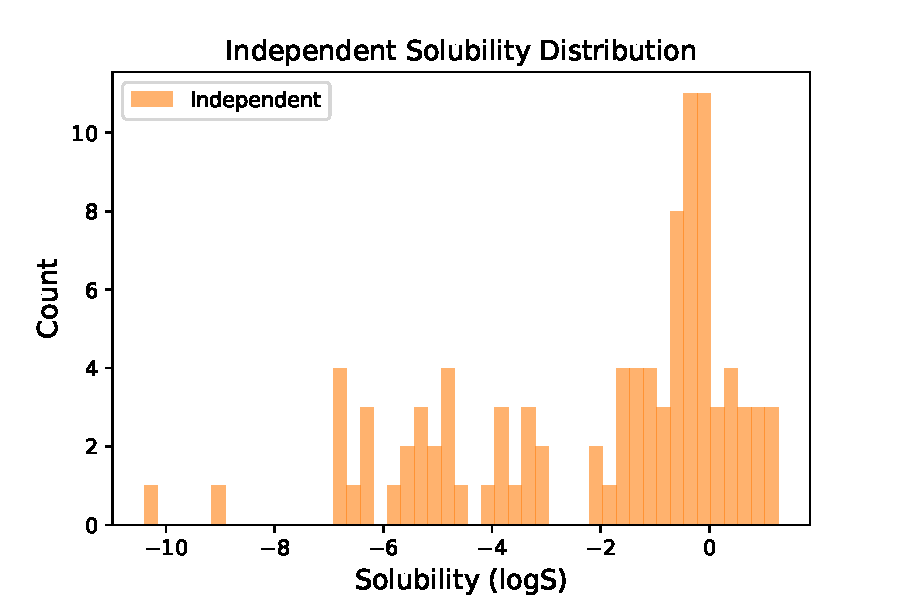
\includegraphics[width=\linewidth]{figures/Independent_solhist.pdf}
    \end{subfigure}
    \caption{Distributions of our various training set data. Each bin has a width of 0.25 units. The first 3 histograms are for the 3 fold scaffold split of AqSolDB, and the last 2 are the full AqSolDB and out independent test set. Note that fold 1 of our scaffold split is particularly challenging as the test set distribution is very different from the training set.}
    \label{fig:solhists}
\end{figure}

\begin{figure}[tb]
    \begin{subfigure}[t]{0.48\textwidth}
        \centering
        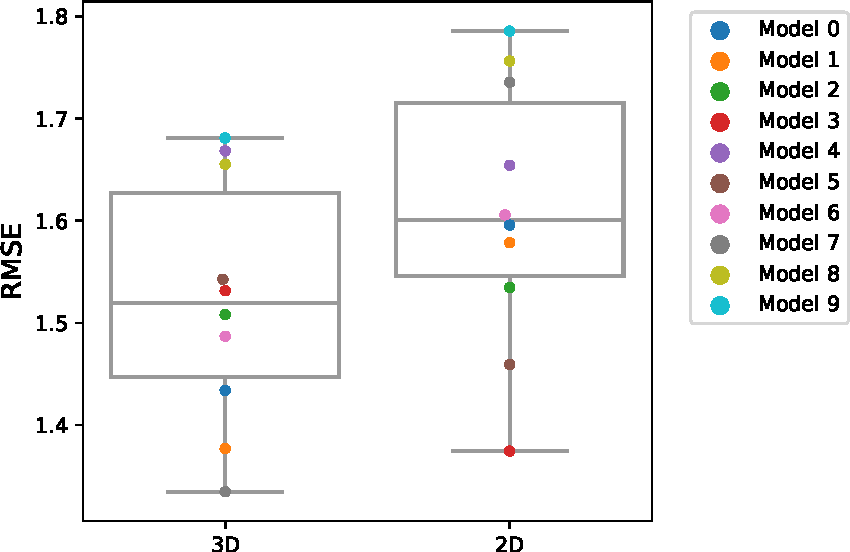
\includegraphics[width=\linewidth]{figures/2dv3d_rmse.pdf}
        \caption{There is no statistically significant difference between these two collections ($p=0.144$), however the mean performance is better for the 3D models (1.522 vs 1.608).}
    \end{subfigure}%
    \hfill
    \begin{subfigure}[t]{0.48\textwidth}
        \centering
        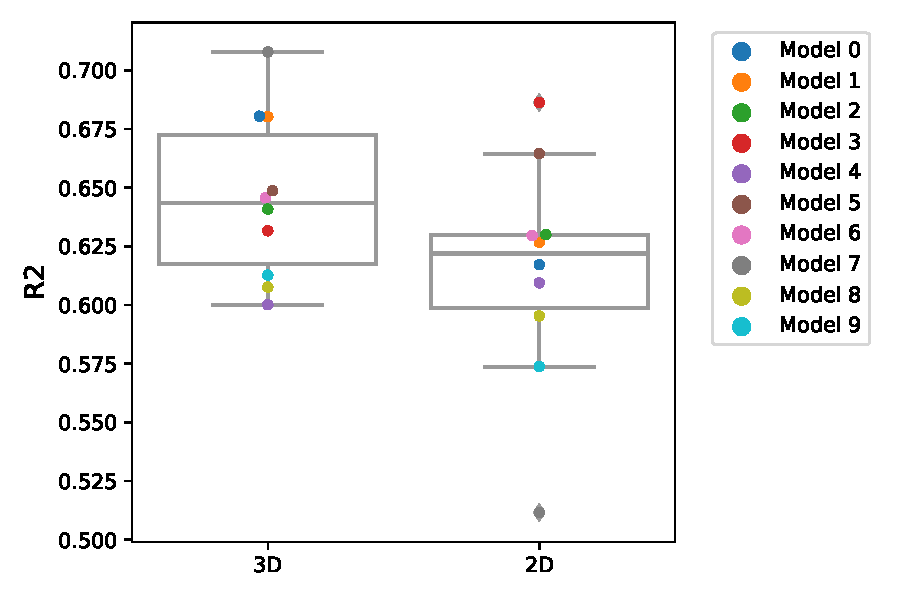
\includegraphics[width=\linewidth]{figures/2dv3d_r2.pdf}
        \caption{There is no statistically significant difference between these two collections ($p=0.116$), but the mean performance of the 3D models is better than the 2D models (0.646 vs 0.614).}
    \end{subfigure}
    \caption{RMSE (a) and $R^2$ (b) performance for the first 10 models trained during the architecture sweep. There is no statistically significant difference between using 2D conformers or 3D conformers for generating the distance matrix used by SolTranNet.}
    \label{fig:2dv3d}
\end{figure}

\begin{figure}[tb]
    \centering
    \begin{subfigure}[t]{0.48\textwidth}
        \centering
        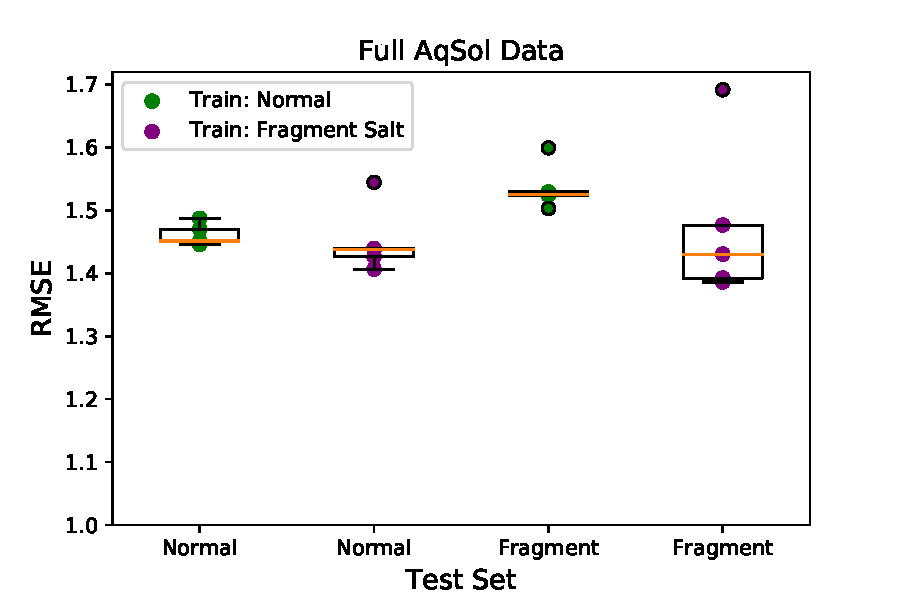
\includegraphics[width=\linewidth]{figures/full_saltfragfirst_RMSEs_boxplots.pdf}
    \end{subfigure}%
    \hfill
    \begin{subfigure}[t]{0.48\textwidth}
        \centering
        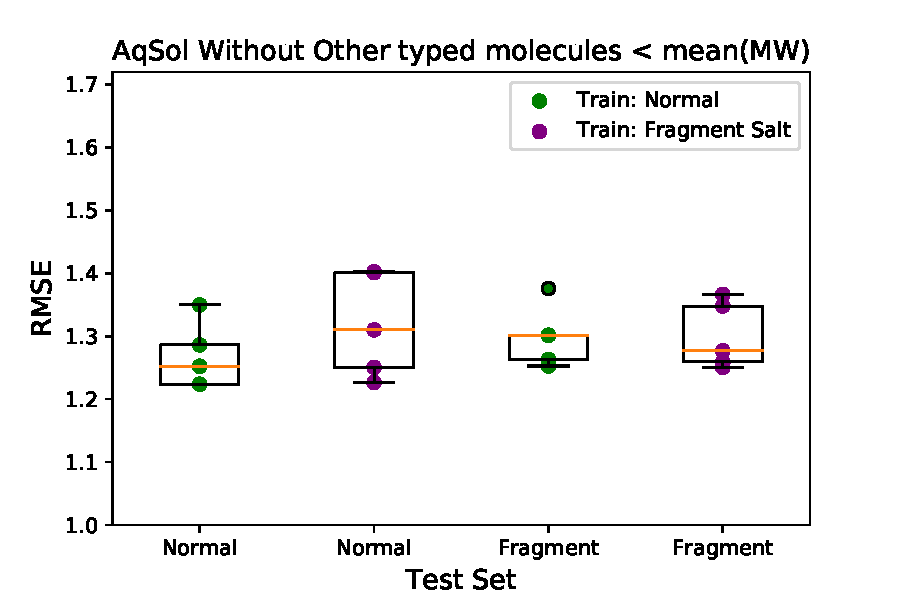
\includegraphics[width=\linewidth]{figures/othersMW_saltfragfirst_RMSEs_boxplots.pdf}
    \end{subfigure}
    
    \begin{subfigure}[t]{0.48\textwidth}
        \centering
        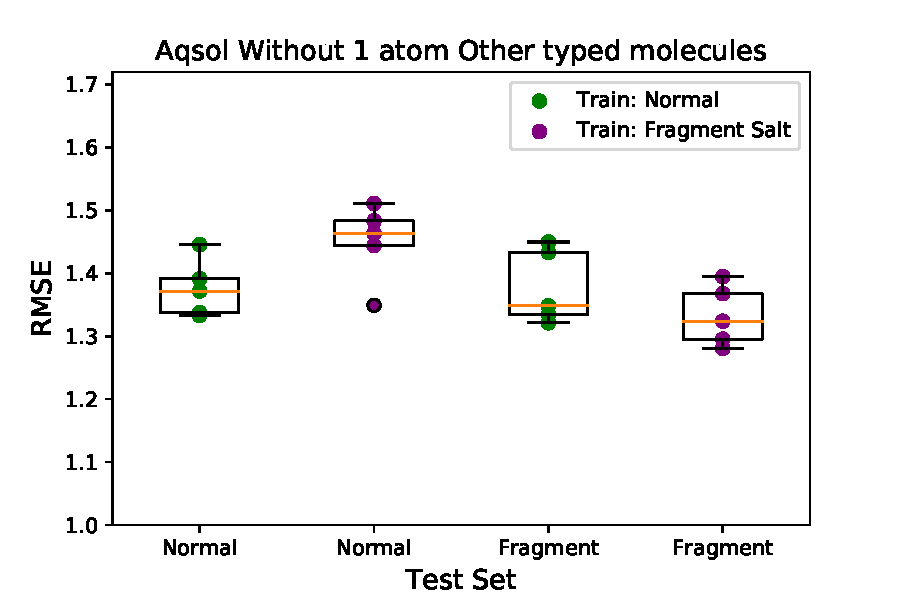
\includegraphics[width=\linewidth]{figures/others2plus_saltfragfirst_RMSEs_boxplots.pdf}
    \end{subfigure}%
    \hfill
    \begin{subfigure}[t]{0.48\textwidth}
        \centering
        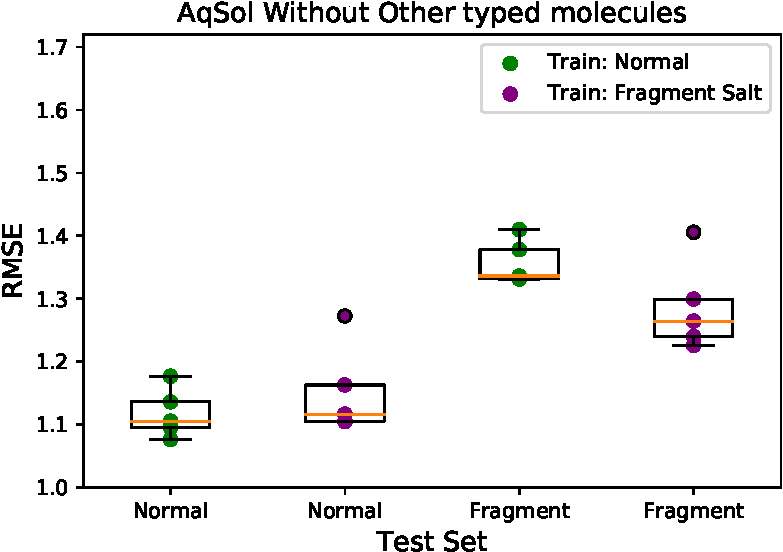
\includegraphics[width=\linewidth]{figures/noothers_saltfragfirst_RMSEs_boxplots.pdf}
    \end{subfigure}
    \caption{RMSE of 5 different SolTranNet trained on the scaffold split of AqSolDB. The horizontal axis is dependent on if the salts were fragmented in the test set, while the colors of the boxplot are dependent on if the salts were fragmented in the training set. Each plot has successively fewer data points in the training and testing sets by more stringently removing atoms which would be embedded as ``Other type'' during training. There is no statistically significant difference in performance on the test set between training on Normal, or Fragmented Salts for all sets.}
    \label{fig:saltfragrmse}
\end{figure}

\begin{figure}[tb]
    \centering
    \begin{subfigure}[t]{0.48\textwidth}
        \centering
        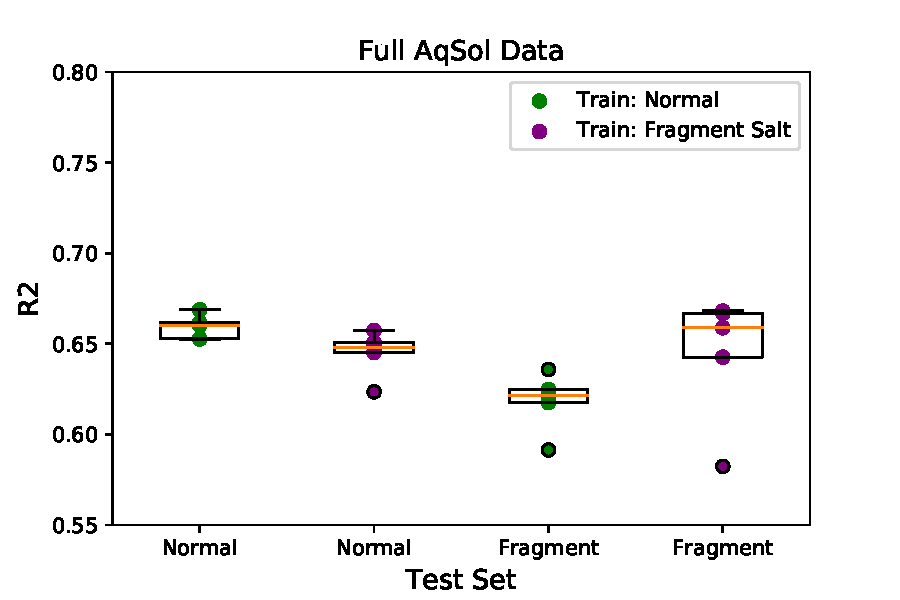
\includegraphics[width=\linewidth]{figures/full_saltfragfirst_R2s_boxplots.pdf}
        \caption{No statistically significant difference between performance on either test set when comparing training with or without fragmented salts ($p=$0.0596 and 0.1852).}
        \label{fig:fullsfr2}
    \end{subfigure}%
    \hfill
    \begin{subfigure}[t]{0.48\textwidth}
        \centering
        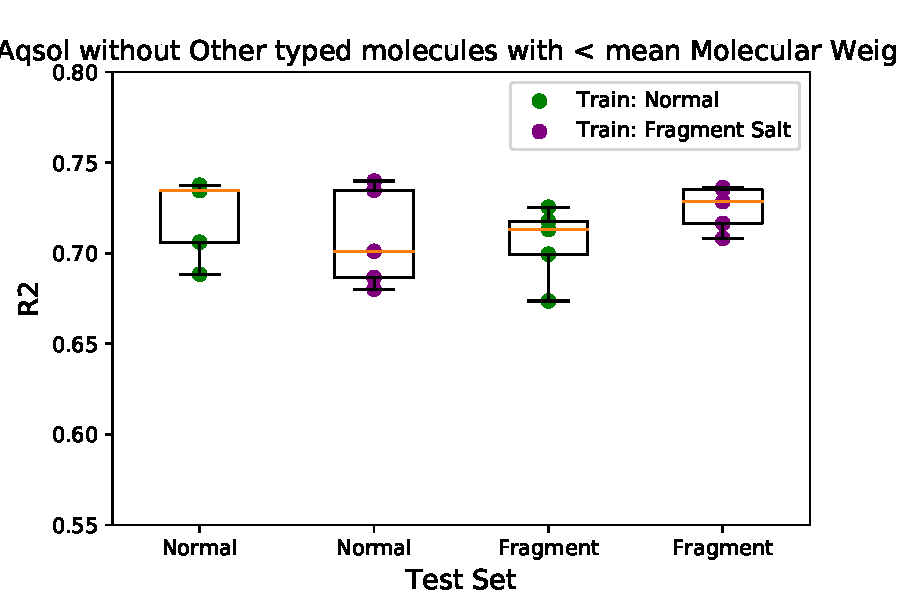
\includegraphics[width=\linewidth]{figures/othersMW_saltfragfirst_R2s_boxplots.pdf}
        \caption{No statistically significant difference between performance on either test set when comparing training with or without fragmented salts ($p=$0.4751 and 0.1100).}
        \label{fig:mwsfr2}
    \end{subfigure}
    
    \begin{subfigure}[t]{0.48\textwidth}
        \centering
        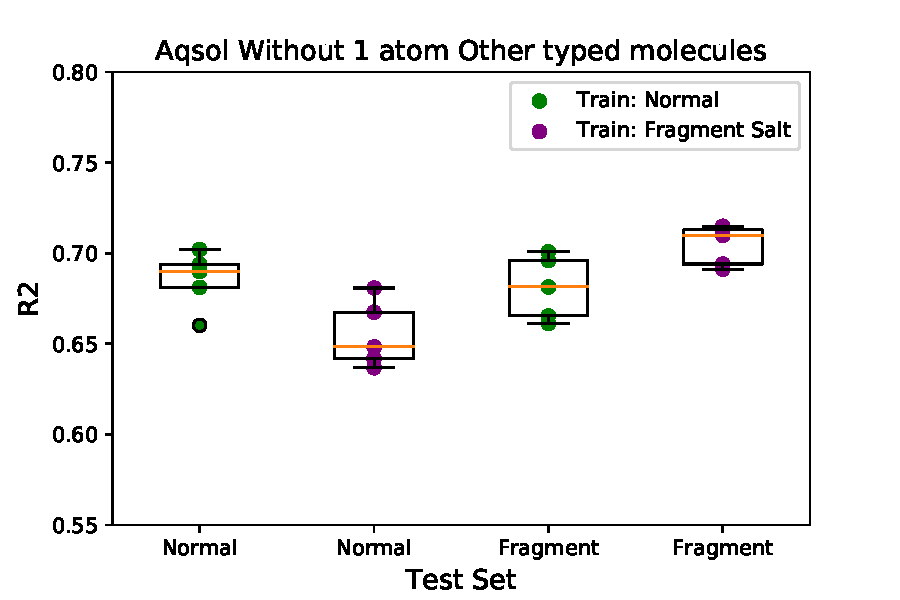
\includegraphics[width=\linewidth]{figures/others2plus_saltfragfirst_R2s_boxplots.pdf}
        \caption{Training with fragmenting salts performed worse on testing on Normal ($p=0.0240$) and better on testing on Fragment ($p=0.03547$).}
        \label{fig:onesfr2}
    \end{subfigure}%
    \hfill
    \begin{subfigure}[t]{0.48\textwidth}
        \centering
        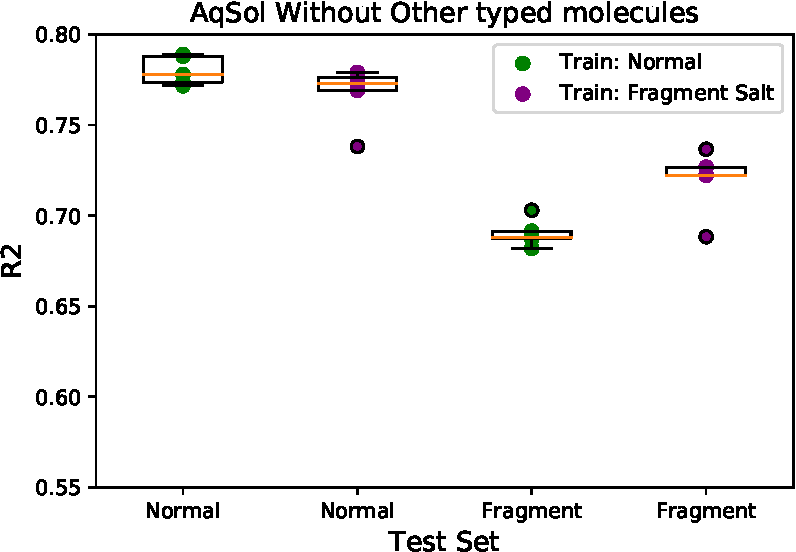
\includegraphics[width=\linewidth]{figures/noothers_saltfragfirst_R2s_boxplots.pdf}
        \caption{Training with fragmented salts had no effect on testing on Normal ($p=0.1555$), but performed better when testing on Fragment ($p=0.0116$).}
        \label{fig:noothersdf2}
    \end{subfigure}
    \caption{$R^2$ of 5 different SolTranNet trained on the scaffold split of AqSolDB. The horizontal axis is dependent on if the salts were fragmented in the test set, while the colors of the boxplot are dependent on if the salts were fragmented in the training set. Each plot has successively fewer data points in the training and testing sets by more stringently removing atoms which would be embedded as ``Other type'' during training.}
    \label{fig:saltfragr2}
\end{figure}


\begin{table}
    \begin{tabular}{|c|c|c|c|c|c|}
        \hline
         Dataset & Reported $R^2$ & Training $R^2$ &  Best $R^2$ & Deployed $R^2$ & Overlap \\
        \hline
        ESOL MAT & -- & 0.911 (0.0151) & -- & -- & 1128/1128 \\
        ESOL STN & -- & 0.915 (0.0106) & -- & 0.890 (0.021) & 1119/1128 \\
        \hline 
         Cui2020 & 0.412 & 0.589(0.0244) & 0.611 &  0.656 & 0/62 \\
        Boobier2017 & 0.706 &  0.543(0.142) & 0.724 &  0.773 & 23/25 \\
        Louvric2020 &  -- & 0.709(0.0537) & 0.783 & 0.744(0.0345) & 151.4/166 \\
        Llinas2020 set1 & 0.62 & 0.496(0.0268) &  0.527 & 0.514 & 79/100 \\
        LLinas2020 set2 & 0.75 & 0.769(0.0346) & 0.824 & 0.726 & 18/32 \\
        \hline
    \end{tabular}
    \caption{Performance of SolTranNet (STN) on other published datasets. For SolTranNet training, we trained 5 different seeds of our final architecture on the provided training and testing splits and report the mean and standard deviation (in parenthesis). The SolTranNet Deployed column is using our final deployed model to predict the provided test set. The final column is the overlap of the provided test set with our deployed model's training set, as no attempt was made to remove molecules present in the test set from the deployed model's training set. Notably the Louvric set had 5 different randomly selected splits for training and testing, which is why there is a mean in the Deployed and Overlap columns.}
    \label{tab:othersetsr2}
\end{table}

\begin{figure}[tb]
    \centering
    \begin{subfigure}[t]{0.33\textwidth}
        \centering
        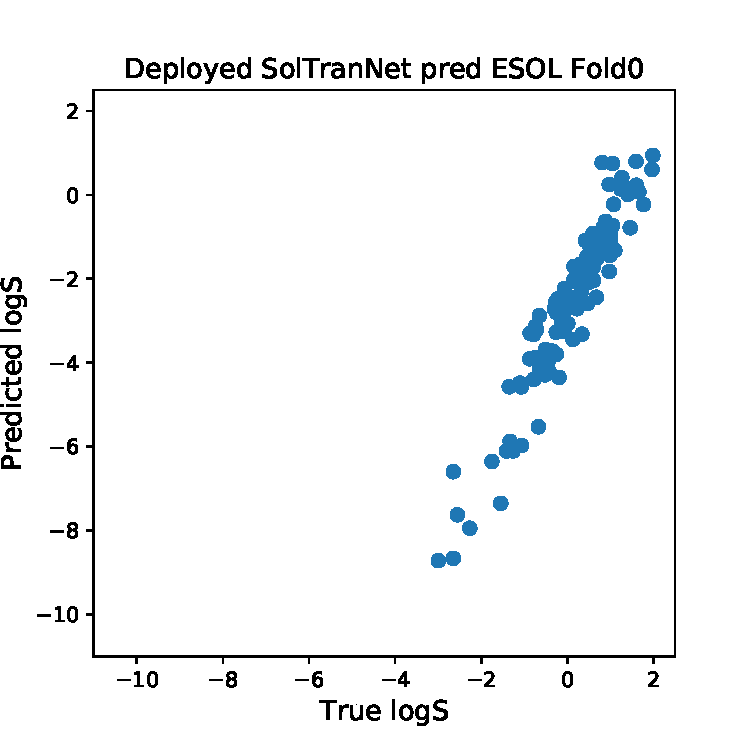
\includegraphics[width=\linewidth]{figures/stn_deployed_pred_esol0.pdf}
    \end{subfigure}%
    \hfill
    \begin{subfigure}[t]{0.33\textwidth}
        \centering
        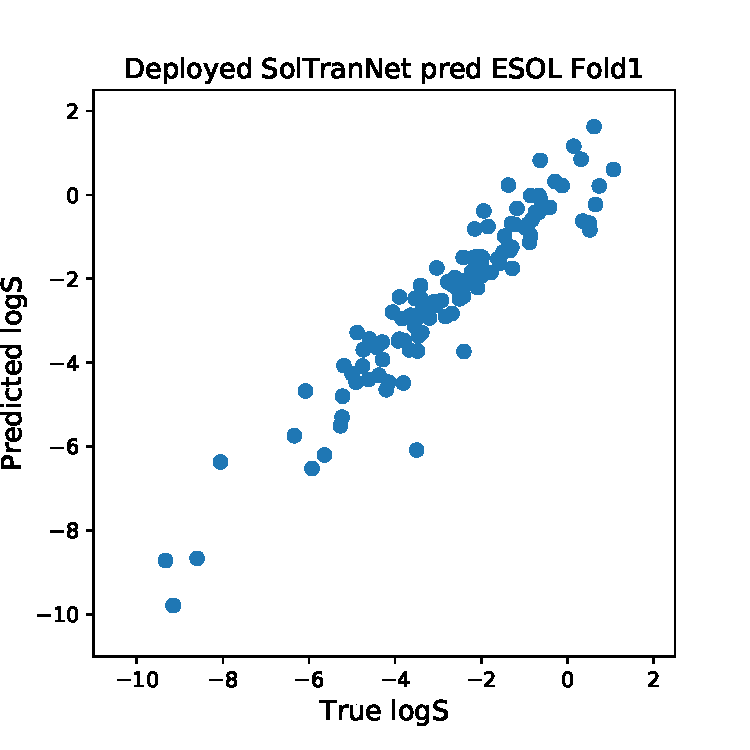
\includegraphics[width=\linewidth]{figures/stn_deployed_pred_esol1.pdf}
    \end{subfigure}%
    \hfill
    \begin{subfigure}[t]{0.33\textwidth}
        \centering
        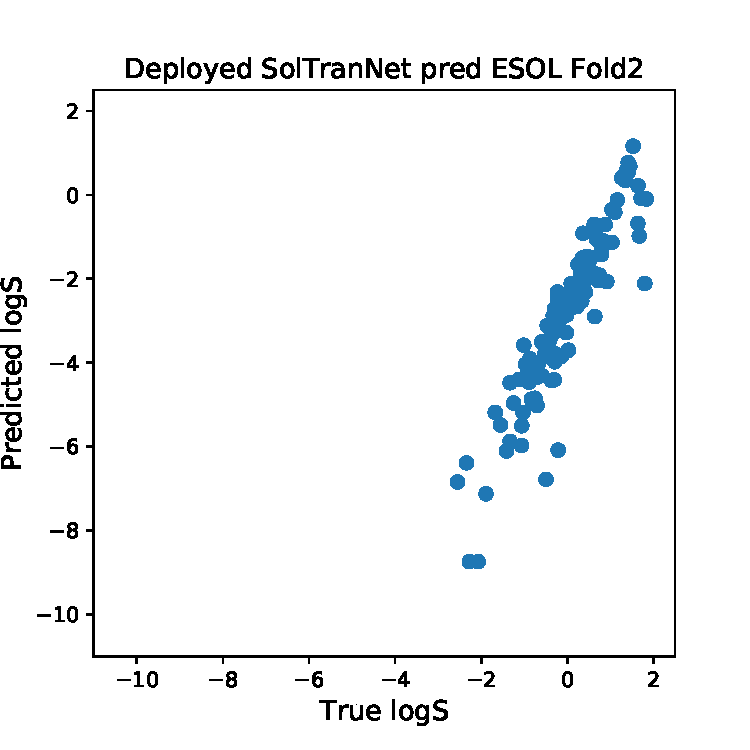
\includegraphics[width=\linewidth]{figures/stn_deployed_pred_esol2.pdf}
    \end{subfigure}
    
    \begin{subfigure}[t]{0.33\textwidth}
        \centering
        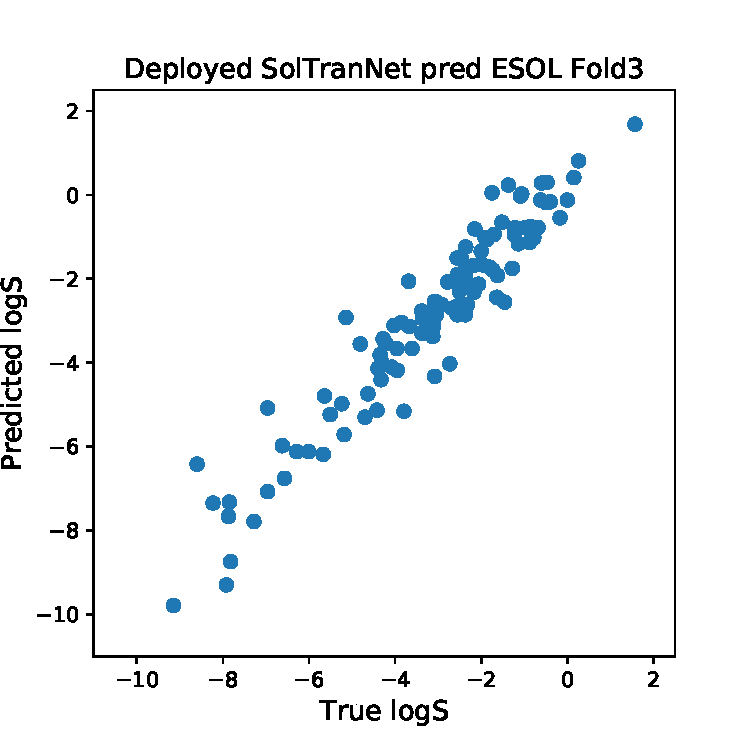
\includegraphics[width=\linewidth]{figures/stn_deployed_pred_esol3.pdf}
    \end{subfigure}%
    \hfill
    \begin{subfigure}[t]{0.33\textwidth}
        \centering
        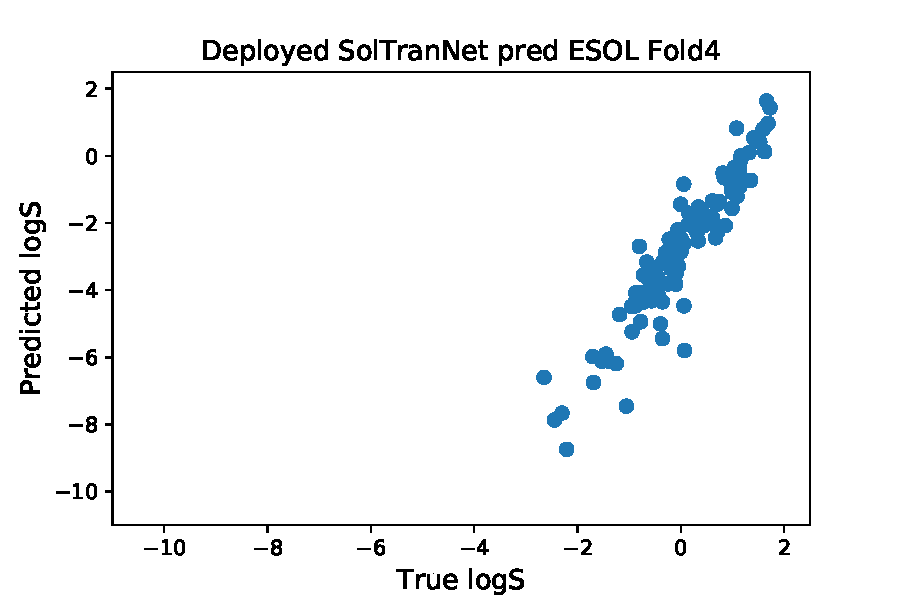
\includegraphics[width=\linewidth]{figures/stn_deployed_pred_esol4.pdf}
    \end{subfigure}%
    \hfill
    \begin{subfigure}[t]{0.33\textwidth}
        \centering
        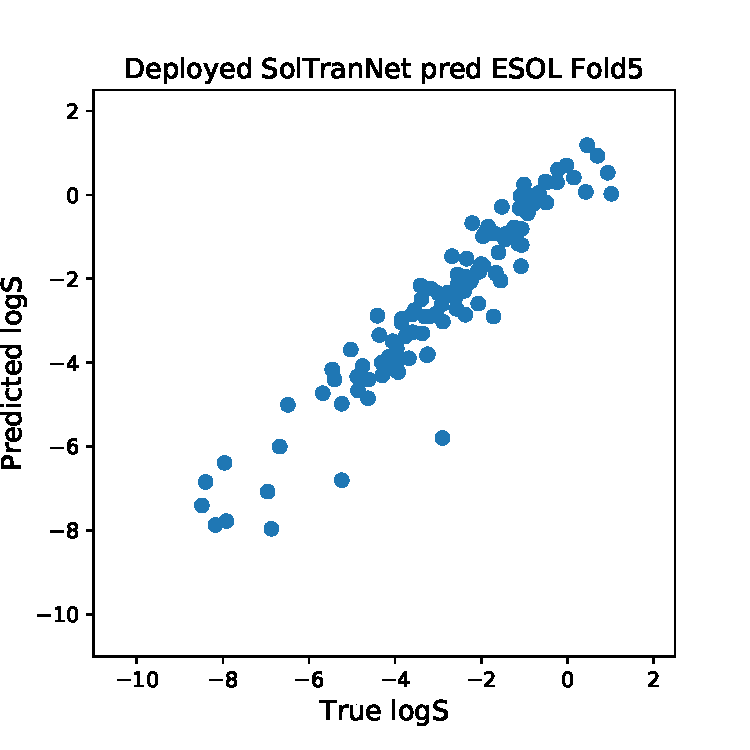
\includegraphics[width=\linewidth]{figures/stn_deployed_pred_esol5.pdf}
    \end{subfigure}
    \caption{Plots of the Deployed SolTranNet model predicting the test sets for each of the random ESOL splits. The predictions have high correlation ($R^2$=0.890), and low RMSE (0.361). Notably, the ESOL data is present in the training set of SolTranNet.}
    \label{fig:stndepesol}
\end{figure}


\begin{figure}[tb]
    \centering
    \begin{subfigure}[t]{0.33\textwidth}
        \centering
        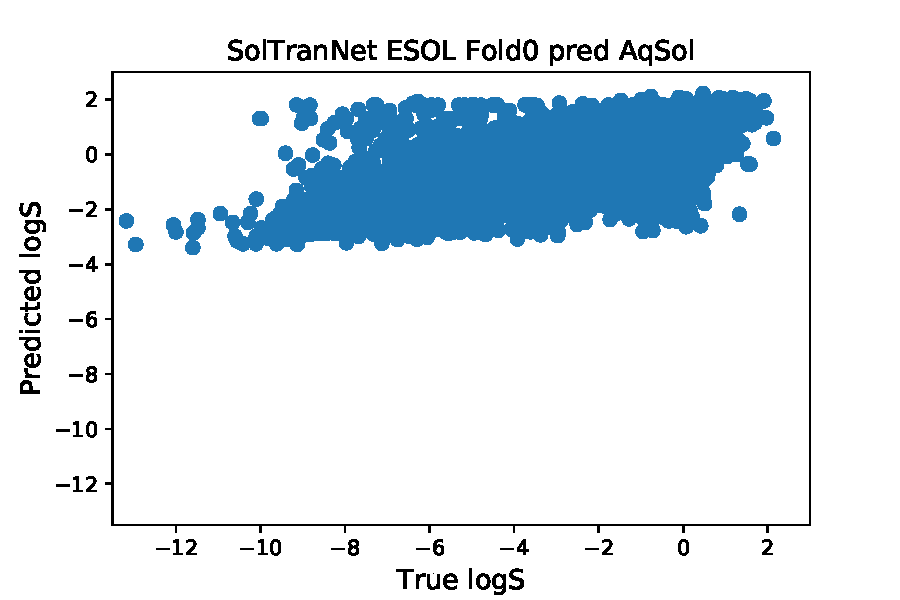
\includegraphics[width=\linewidth]{figures/stn_esol0_pred_aqsol.pdf}
    \end{subfigure}%
    \hfill
    \begin{subfigure}[t]{0.33\textwidth}
        \centering
        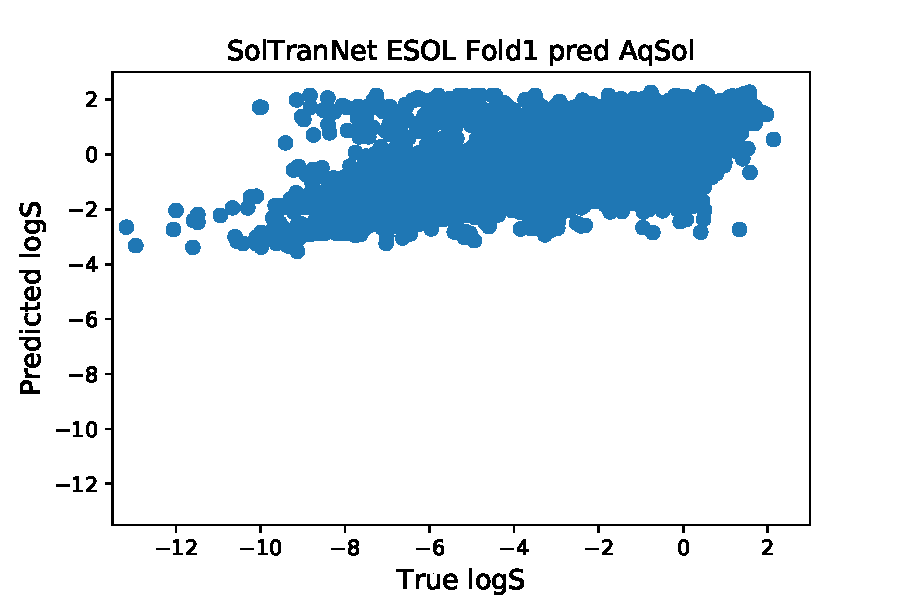
\includegraphics[width=\linewidth]{figures/stn_esol1_pred_aqsol.pdf}
    \end{subfigure}%
    \hfill
    \begin{subfigure}[t]{0.33\textwidth}
        \centering
        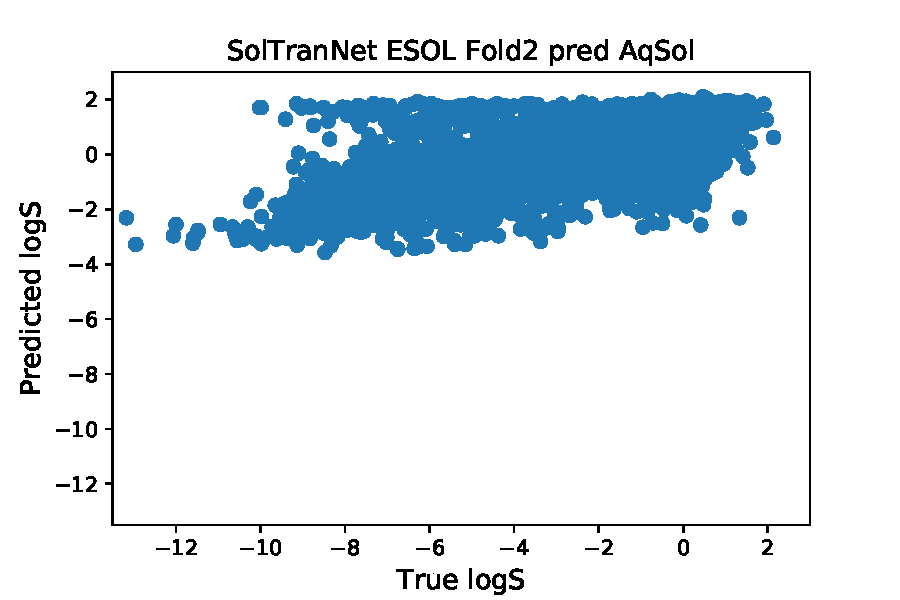
\includegraphics[width=\linewidth]{figures/stn_esol2_pred_aqsol.pdf}
    \end{subfigure}
    
    \begin{subfigure}[t]{0.33\textwidth}
        \centering
        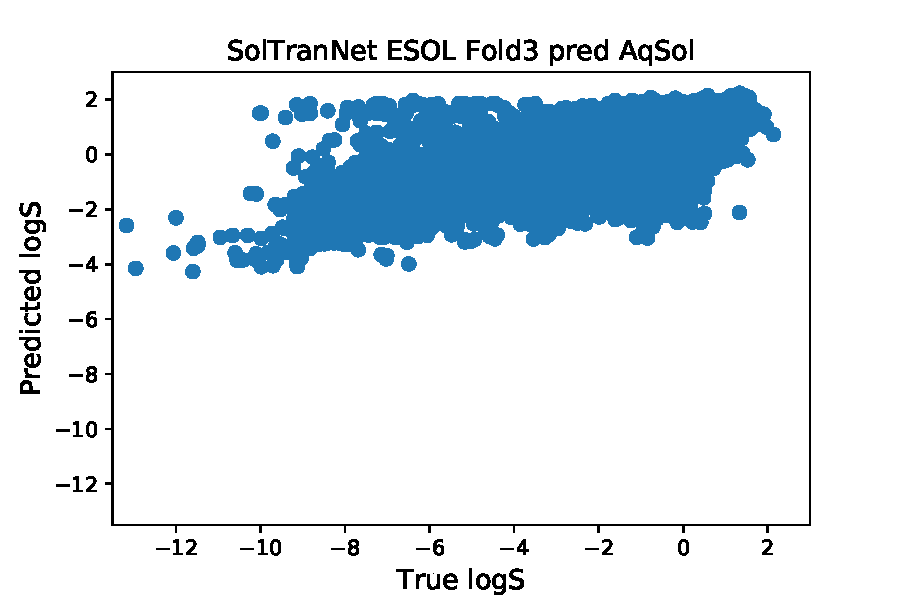
\includegraphics[width=\linewidth]{figures/stn_esol3_pred_aqsol.pdf}
    \end{subfigure}%
    \hfill
    \begin{subfigure}[t]{0.33\textwidth}
        \centering
        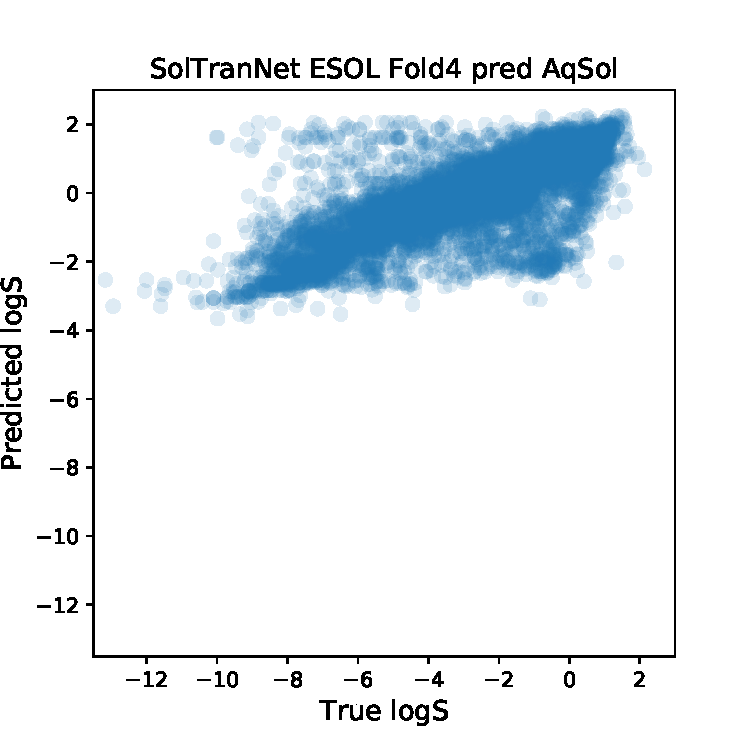
\includegraphics[width=\linewidth]{figures/stn_esol4_pred_aqsol.pdf}
    \end{subfigure}%
    \hfill
    \begin{subfigure}[t]{0.33\textwidth}
        \centering
        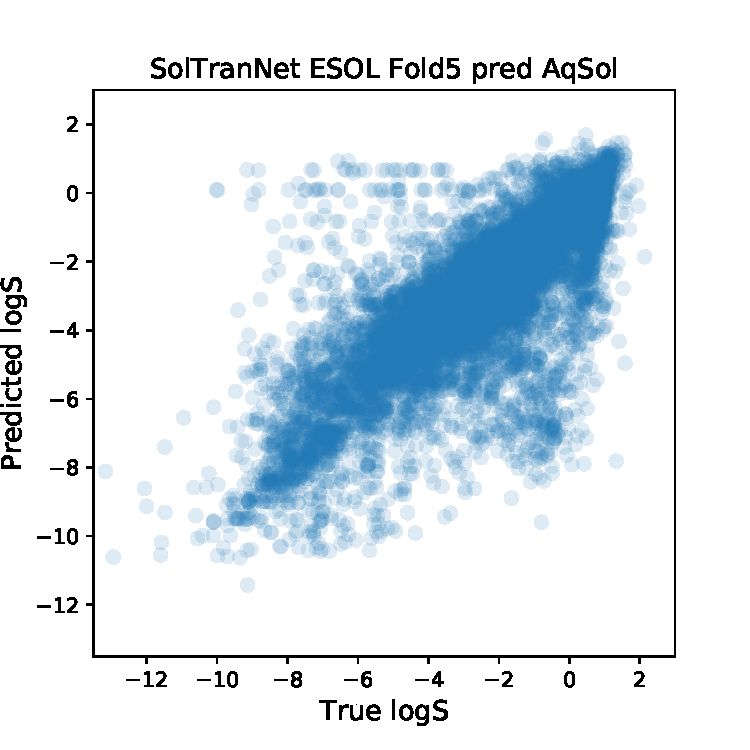
\includegraphics[width=\linewidth]{figures/stn_esol5_pred_aqsol.pdf}
    \end{subfigure}
    \caption{Plots of SolTranNet trained on the random splits of ESOL predicting AqSol. The predictions have low correlation ($R^2=0.552$), and high RMSE (1.67).}
    \label{fig:stnesolaqsol}
\end{figure}

\begin{figure}[tb]
    \centering
    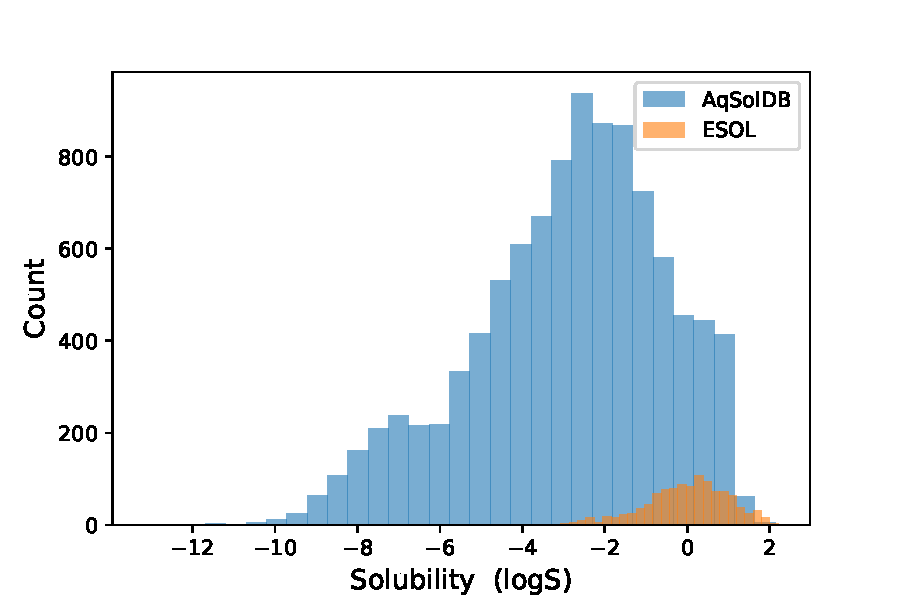
\includegraphics{figures/esol_stn_hist.pdf}
    \caption{Training distributions of AqSol (blue) and ESOL (orange). Bin width is half a log unit. Notably, the distribution of solubilities in AqSol is markedly different than the distribution of solubilities in ESOL.}
    \label{fig:esol_hist}
\end{figure}

\begin{table}
    \centering
    \begin{tabular}{|c|c|c|c|}
    \hline
        Training Set & Testing Set & RMSE & $R^2$ \\
    \hline
        ESOL* & AqSol & 1.67 (0.021) & 0.552 (0.0062) \\
        AqSol & AqSol & 1.16 & 0.77 \\
    \hline
    \hline
        AqSol & ESOL & 0.361 (0.017) & 0.89 (0.021) \\
        ESOL & ESOL & 0.289 (0.011) & 0.915 (0.011) \\
    \hline    
    \end{tabular}
    \caption{SolTranNet comparison of performance utilizing ESOL or AqSol on predicting logS. Models tested on AqSol are tested on the entire AqSol dataset. Thus the AqSol-AqSol model is simply reporting its performance on its own training set (and is only a singular model). The models utilizing ESOL are either training or testing on the 6 provided random splits of ESOL from the original MAT publication. Note that these values were mean centered and normalized in the original MAT dataset, but have been transformed back to logS units. We report the mean performance, with the standard deviation in parenthesis. Note, no attempt was made to remove molecules present in the test set from the training set. You can see the predictions for the swapped sets in Fig~\ref{fig:stndepesol}-\ref{fig:stnesolaqsol} and the histogram of the solubilites in AqSol and ESOL in Fig~\ref{fig:esol_hist}. Notably, models trained with either set and tested on the other exhibit worse RMSE. However, models trained on ESOL fail to generalize their predictions to the broader range of molecules present in AqSol, which contributes to the low $R^2$ of their predictions and worse RMSE. This leads to a model trained on ESOL to be less useful as a screen, since it is likely to misclassify soluble molecules. The reverse situation does not occur, where a model trained on AqSol maintains a high Pearson's $R^2$ on ESOL, which makes it more suitable in a screening context.}
    \label{tab:esolaqsol}
\end{table}
\end{document}